\documentclass[12pt,a4paper]{report}
\usepackage[utf8]{inputenc}
\usepackage[frenchb]{babel}
%\usepackage{baskervald}
\usepackage{gfsartemisia}
%\usepackage{palatino}
%\usepackage{libertine}
\usepackage[T1]{fontenc}
\usepackage{textcomp} % Pour les symboles spéciaux
\usepackage{listings} % Pour l'ajout de code source
\usepackage{graphicx} % Pour l'ajout des images
\usepackage{titlesec} % Pour ne plus avoir le mot chapitre
\usepackage{lettrine} % Pour l'usage des lettrines

% Pas de mot 'chapitre'
\titleformat{\chapter}[hang]{\bf\huge}{\thechapter}{2pc}{}

% Marge pour la reliure
\addtolength{\hoffset}{+0.5cm}

% Style de page personalisé%{{{
\usepackage{fancyhdr}
\pagestyle{fancy} % Ceci permet d’avoir les noms de chapitre et de section % en minuscules
\renewcommand{\chaptermark}[1]{\markboth{#1}{}}
\renewcommand{\sectionmark}[1]{\markright{\thesection\ #1}}
\fancyhf{}	% supprime les en-têtes et pieds
\fancyhead[LE,RO]{\bfseries\thepage}% Left Even, Right Odd
\fancyhead[LO]{\bfseries\rightmark} % Left Odd
\fancyhead[RE]{\bfseries\leftmark} % Right Even
\renewcommand{\headrulewidth}{0.5pt}% filet en haut de page
\addtolength{\headheight}{0.5pt}	% espace pour le filet
\renewcommand{\footrulewidth}{0pt} % pas de filet en bas
\fancypagestyle{plain}{ % pages de tetes de chapitre
\fancyhead{}	% supprime l’entete
\renewcommand{\headrulewidth}{0pt} % et le filet
}%}}}

%Couverture%{{{

\title
{
	\normalsize{Lycée Jean Bart - Dunkerque\\
	2011-2012}\\
	\vspace{15mm}
  \LARGE{Création d'un serveur Web personnalisé ainsi que sa mise en
    \oe{}uvre avec une application IdentIt chez un client et mise en
    place de Git
    \vspace{15mm}}
}
\author{\bsc{Stechele} Julien\\
	\vspace{35mm}
}

\date{
	\normalsize{Entreprise d'accueil : IdentIt\\
    route du Pont Noir - Port 2122\\
  Dunkerque\\
	\vspace{5mm}
  Tuteur de stage : \bsc{M.~Anselin}\\
	Maître de stage : \bsc{M.~Dubourg}
	}
}%}}}

\begin{document}%{{{

\maketitle

\chapter*{Remerciements} % (fold)
\label{cha:Remerciements}

\lettrine{J}{e} tiens à remercier :
\begin{itemize}
    \item \bsc{M.~Dubourg} pour le suivi qu'il m'a apporté pendant toute la
    durée des stages, le temps qu'il m'a consacré pour m'initier à la
    programmation orientée objet, les astuces techniques pour développer
    plus rapidement ainsi que l'enseignement des habitudes propres à
    l'entreprise ;
    \item La société IdentIt pour avoir accepté ma candidature, j'espère avoir
    été à la hauteur de leurs attentes ;
    \item Les développeurs pour m'avoir aiguillé quand j'étais en détresse ;
    \item L'équipe enseignante pour nous avoir appris les fondements du
    développement et l'univers informatique tout autour qui en découle.
\end{itemize}
% chapter Remerciements (end)


% Pour écrire Sommaire au lieu de table des matières
\renewcommand{\contentsname}{Sommaire}

% Interligne pour le sommaire
{\setlength{\baselineskip}{2.3\baselineskip}\tableofcontents\par}

\chapter{Introduction} % (fold)
\label{cha:Introduction}

\lettrine{J}{e} m'appelle Julien \bsc{Stechele}, je suis actuellement en
BTS\, \footnote{\emph{Brevet de Technicien Supérieur.}} informatique de
gestion option développeur d'applications et dans le cadre de mes études
j'ai la chance d'effectuer deux stages durant cette formation. Mon stage
de première année s'est déroulé du 16 mai 2011 au 8 juillet 2011 dans la
société \emph{IdentIt} ainsi que mon deuxième stage qui lui s'est
déroulé du 3 janvier 2012 au 21 février 2012. C'est une SARL\,
\footnote{\emph{Société À Responsabilité Limitée.}} de quatre personnes
qui se situe à Petite-Synthe. \bsc{M.~Dubourg} et \bsc{M.~Lesage} sont
les fondateurs de cette structure, le premier s'occupe de la partie
technique en tant que chef de projet et le second de la partie gestion
de l'entreprise. Ils sont accompagnés par deux développeurs, l'un
travaillant sur la partie application sur Windows
Mobile~\textregistered, l'autre sur la partie internet.

Mon premier travail consistait à développer un utilitaire pour la partie
web de comparaison de bases de données qui permetterait d'améliorer le
suivi des mises à jour d'une base obsolète à partir d'une base de
référence et aussi de fournir les requêtes permettant cette mise à jour.
Mon deuxième travail était de mettre en place un nouvel outil de gestion
de version de code source plus évolué que l'existant.

Mon deuxième stage, qui est l'objet de cette note de synthèse, consiste
à continuer le travail précédent sur le gestionnaire de version puis à
crée un serveur Web dérivée d'un logiciel libre existant pour ensuite le
déployer avec une application d'IdentIt chez un client, le tout en
s'accordant avec le système d'information de l'acquéreur.

Cette note de synthèse suit un plan spécifique, mais les événements ne
se sont pas passés dans l'ordre réel. En effet, à cause des difficultés
rencontrées et des problématiques nouvelles données en cours de stage,
je suis souvent passé d'une réalisation à une autre.
% chapter Introduction (end)


% L'entreprise
\chapter{L'entreprise} % (fold)
\label{cha:L'entreprise}

% chapter L'entreprise (end)


% La gestion de version
\chapter{Création d'IITAMP} % (fold)
\label{cha:Création d'IITAMP}

\begin{it}
  La majeur partie des entreprises utilisant l'informatique
  dispose d'un réseau local. Le but de IITAMP\, \footnote{\emph{IdentIt
  Apache MySQL PHP.}} est de fournir les outils capables de faire
  fonctionner une application Web développé par \emph{IdentIt} sur un
  poste informatique d'une entreprise de façon simple et efficace, ce
  qui permet de ce passer d'un hébergeur sur internet et d'autres
  avantages.
\end{it}

\section{Les avantages d'un intranet} % (fold)%{{{
\label{sec:Les avantages d'un intranet}

\lettrine{C}{ertaines} entreprises dans un but de confidentialité
préfèrent utiliser des applications en intranet. Dans mon cas, un
serveur sous Windows Server 2008 utilise IITAMP ainsi
qu'une application \emph{IdentIt} pour qu'a partir du réseau local tout
les ordinateurs puissent utiliser l'application. De ce fait, le produit
n'est pas accessible via l'Internet.

La confidentialité n'est pas le seul atout. En effet, passer par un
réseau d'entreprise en terme de performance est avantageux car les
requêtes entre le client et le serveur ce font \emph{intra muros} tandis
que passer par un hébergeur qui peut ce trouver à des milliers de
kilomètres affecte les délais. Utiliser une solution d'hébergement sur
le réseau des réseaux à un coût alors qu'une solution locale n'est pas
forfaitaire.

Dans le cas d'un hébergement, si la connexion à internet vient à être
interrompu, le service n'est plus disponible. Par contre avec notre
solution ça continue à fonctionner.
% section Les avantages d'un intranet (end)%}}}

\section{La base applicative} % (fold)%{{{
\label{sec:La base applicative}

Je suis tout d'abord parti d'une base XAMPP générique. C'est un logiciel
libre développé par une équipe de bénévoles. Cette ensemble de
programmes permettent de mettre en \oe{}uvre un serveur web sur un PC
Windows à des fins de développement. La suite XAMPP regroupe les
logiciels Apache\, \footnote{Serveur HTTP}, MySQL\, \footnote{Serveur de
base de données.} et PHP\, \footnote{\emph{PHP: Hypertext Preprocessor}
acronyme récursif désignant un langage de script.}. De ce fait, il
permet d'héberger sur la machine qui la compose un site internet
dynamique. La solution de base ne nous satisfaisant pas, mon travail
consista à modifier ce gratuiciel pour les besoins de déploiement des
produits \emph{IdentIt}.
% section La base applicative (end)%}}}

\section{Les objectifs} % (fold)%{{{
\label{sec:Les objectifs}

\subsection{La maintenabilité} % (fold)%{{{
\label{sub:La maintenabilité}

Pour proposer une maintenance de bug efficace est facile il a fallut
installer le module PHP \emph{Xdebug} qui permet d'afficher des erreurs
plus significatives que celles de PHP par défaut. En effet, celui-ci
permet la coloration syntaxique ainsi que les valeurs des variables qui
précède le bug. J'ai aussi externalisé les fichiers d'historique dans un
dossiers séparé ce qui permet d'y accéder facilement. Auquel cas on
puisse demander au client de nous envoyer le dossier archivé par
courrier électronique pour analyser si Xdebug ne suffisait pas pour
d'écrire l'erreur rencontré par téléphone.
% subsection La maintenabilité (end)%}}}

\subsection{L'évolutivité} % (fold)%{{{
\label{sub:L'évolutivité}

Comme les dossiers sont séparés méticuleusement, une mise à jour de
l'applicatif web ou du serveur IITAMP ce fait à partir en quelques
étapes très simple contrairement au logiciel de base qui aurait
nécessité beaucoup de manipulation, la plus pars de ses interventions
étant demander au client lorsque les applications seront misent en
production.
% subsection L'évolutivité (end)%}}}

\subsection{La pérennité des données} % (fold)
\label{sub:La pérennité des données}

La informations des bases de données ainsi que les informations du
navigateur Web sont extraite du dossier IITAMP ce qui permet de faire
une sauvegarde efficace de celles-ci. La sauvegarde ce fait à partir
d'une tache journalière que j'ai décrite dans un document pour
l'utilisateur.
% subsection La pérennité des données (end)

\subsection{L'éfficacité} % (fold)%{{{
\label{sub:L'éfficacité}

Pour optimiser le serveur IITAMP, une inspection profonde du logiciel
fut nécessaire. En effet, celui-ci est composé de base d'une multitude de
librairies et modules qui ne sont pas forcement utile au applications
développé par \emph{IdentIt}. De ce fait, un nettoyage fut entrepris. Un
gain de 20 mega-octets à été constaté.
% subsection L'éfficacité (end)%}}}

\subsection{La simplicité} % (fold)%{{{
\label{sub:La simplicité}

Pour rendre simple l'utilisation du serveur web pour le client, il à
fallut créer des scripts d'automatisations pour certaines taches pas
forcements évidentes pour les non initiés. Par exemple l'installation des
applications entant que services ainsi que le démarrage des dit services.
J'ai aussi développer une page d'index dans le cas ou le client à
plusieurs applications web de l'entreprise \emph{IdentIt}, auquel cas une
sélection de l'application est a faire.
% subsection La simplicité (end)%}}}

\subsection{La propriété} % (fold)%{{{
\label{sub:La propriété}

Pour la partie juridique dans un soucis de propriété intellectuelle,
j'ai installé un module qui permet le chiffrement du code source PHP,
cette extension s'appelle Bcompiler et m'a servi lors de l'installation
des applications après la finalisation du serveur IITAMP.
% subsection La propriété (end)%}}}
% section Les objectifs (end)%}}}

\section{Les documentations} % (fold)%{{{
\label{sec:Les documentations}

\begin{description}

  \item[Création d'un IITAMP :] Permet de recréer un serveur IITAMP à
    partir d'un serveur XAMPP qui incorpore des nouveautés ou des mises
    à jours.

  \item[Mise en \oe{}uvre d'un IITAMP :] mise en place de l'IITAMP
    nouvellement installé en entreprise ou mise à jour de celui-ci.

  \item[Construction d'une application Web :] Permet de guider la
    préparation d'une application Web d'\emph{IdentIt} pour quel soit
    parfaitement intégré à IITAMP.

  \item[Déploiement d'une application Web :] Comment mettre en place ou
    mettre à jour une application web dans un IITAMP déjà en service.

  \item[Maintenance de bases de données :] Explication de la mise en
    place d'une sauvegarde automatique des bases de données des
    applications ainsi que la restauration de ses sauvegardes.

  \item[Démarche d'activation d'une application GeMa :] Documentation
    pour \emph{IdentIt} compréhensible par les non techniciens qui
    explique comment activer une application chez un client.

  \item[Mise en place de GeMa en entreprise :] Documentation pour les
    clients qui décrit les premières étapes à suivre pour utiliser GeMa.

\end{description}
% section Les documentations (end)%}}}
% chapter Création d'IITAMP (end)


% Création d'IITAMP
\chapter{Création d'IITAMP} % (fold)
\label{cha:Création d'IITAMP}

\begin{it}

  La majeure partie des entreprises utilisant l'informatique disposent
  d'un réseau local. Le but de IITAMP\, \footnote{\emph{IdentIt Apache
  MySQL PHP.}} est de fournir les outils capables de faire fonctionner
  une application Web développée par \emph{IdentIt} sur un poste
  informatique d'une entreprise de façon simple et efficace, ce qui
  permet de se passer d'un hébergeur sur internet et de bénéficier
  d'autres avantages.

\end{it}

\section{Les avantages d'un intranet} % (fold)%{{{
\label{sec:Les avantages d'un intranet}

\lettrine{C}{ertaines} entreprises, dans un but de confidentialité
préfèrent utiliser des applications en intranet. Dans le cadre de mon
stage, un serveur sous Windows Server 2008 utilise IITAMP ainsi qu'une
application d'\emph{IdentIt} pour qu'à partir du réseau local tous les
ordinateurs puissent utiliser l'application. De ce fait, le produit
n'est pas accessible via Internet.

La confidentialité n'est pas le seul atout. En effet, passer par un
réseau d'entreprises en terme de performance est avantageux car les
requêtes entre le client et le serveur se font \emph{intra muros} ;
alors que passer par un hébergeur qui peut se trouver à des milliers de
kilomètres affecte les délais. Utiliser une solution d'hébergement sur
le réseau des réseaux a un coût alors qu'une solution locale n'est pas
forfaitaire.

Dans le cas d'un hébergement, si la connexion à internet vient à être
interrompue, le service n'est plus disponible. Par contre, avec notre
solution cela continue de fonctionner.
% section Les avantages d'un intranet (end)%}}}

\section{La base applicative} % (fold)%{{{
\label{sec:La base applicative}

Je suis tout d'abord parti d'une base XAMPP générique. Il s'agit d'un
logiciel libre développé par une équipe de bénévoles. Cet ensemble de
programmes permet de mettre en \oe{}uvre un serveur web sur un PC
Windows à des fins de développement. La suite XAMPP regroupe les
logiciels Apache\, \footnote{Serveur HTTP}, MySQL\, \footnote{Serveur de
base de données.} et PHP\, \footnote{\emph{PHP: Hypertext Preprocessor}
acronyme récursif désignant un langage de script.}. De ce fait, il
permet d'héberger sur la machine qui la compose un site internet
dynamique. La solution de base ne nous satisfaisant pas, mon travail
consista à modifier ce gratuiciel pour les besoins de déploiement des
produits \emph{IdentIt}.
% section La base applicative (end)%}}}

\section{Les objectifs} % (fold)%{{{
\label{sec:Les objectifs}

\subsection{La maintenabilité} % (fold)%{{{
\label{sub:La maintenabilité}

Pour proposer une maintenance de bug efficace et facile, il a fallu
installer le module PHP \emph{Xdebug} qui permet d'afficher des erreurs
plus significatives que celles de PHP par défaut. En effet, celui-ci
permet la coloration syntaxique ainsi que l'affichage des valeurs des
variables qui précèdent le bug. J'ai aussi externalisé les fichiers
d'historique dans un dossier séparé, ce qui permet un accès plus facile
dans le cas où il faudrait demander au client de nous envoyer le dossier
archivé par courrier électronique pour l'analyser si Xdebug ne suffisait
pas pour décrire l'erreur rencontrée par téléphone.
% subsection La maintenabilité (end)%}}}

\subsection{L'évolutivité} % (fold)%{{{
\label{sub:L'évolutivité}

Comme les dossiers sont séparés méticuleusement, une mise à jour de
l'applicatif web ou du serveur IITAMP se fait à partir de quelques
étapes très simples contrairement au logiciel de base qui aurait
nécessité beaucoup de manipulations, la pluspart de ces interventions
étant demandées au client lorsque les applications seront mises en
production.
% subsection L'évolutivité (end)%}}}

\subsection{La pérennité des données} % (fold)%{{{
\label{sub:La pérennité des données}

Les informations des bases de données ainsi que celles du navigateur Web
sont extraites du dossier IITAMP ce qui permet de faire une sauvegarde
efficace de celles-ci. La sauvegarde se fait à partir d'une tache
journalière que j'ai décrite dans un document pour l'utilisateur.
% subsection La pérennité des données (end)%}}}

\subsection{L'efficacité} % (fold)%{{{
\label{sub:L'efficacité}

Pour optimiser le serveur IITAMP, une inspection profonde du logiciel
fut nécessaire. En effet, celui-ci est composé de base d'une multitude
de librairies et modules qui ne sont pas forcément utiles aux
applications développées par \emph{IdentIt}. De ce fait, un nettoyage
fut entrepris. Un gain de 20 méga-octets a été constaté.
% subsection L'efficacité (end)%}}}

\subsection{La simplicité} % (fold)%{{{
\label{sub:La simplicité}

Pour rendre simple l'utilisation du serveur web pour le client, il a
fallu créer des scripts d'automatisation pour certaines tâches qui
n'étaient pas forcément évidentes pour les non-initiés. Par exemple
l'installation des applications en tant que services ; ainsi que le
démarrage des dit services.  J'ai également développé une page d'index
au cas où le client aurait plusieurs applications web de l'entreprise
\emph{IdentIt}, auquel cas, une sélection de l'application est à faire.
% subsection La simplicité (end)%}}}

\subsection{La propriété} % (fold)%{{{
\label{sub:La propriété}

Pour la partie juridique, dans un souci de propriété intellectuelle,
j'ai installé un module qui permet le chiffrement du code source PHP,
cette extension s'appelle Bcompiler et m'a servi lors de l'installation
des applications après la finalisation du serveur IITAMP.
% subsection La propriété (end)%}}}
% section Les objectifs (end)%}}}

\section{Les documentations} % (fold)%{{{
\label{sec:Les documentations}

\begin{description}

  \item[Création d'un IITAMP :] Permet de recréer un serveur IITAMP à
    partir d'un serveur XAMPP qui incorpore des nouveautés ou des mises
    à jour.

  \item[Mise en \oe{}uvre d'un IITAMP :] mise en place de l'IITAMP
    nouvellement installé en entreprise ou mise à jour de celui-ci.

  \item[Préparation d'une application :] Illustre les étapes de
    préparation d'une application Web d'\emph{IdentIt} pour qu'elle soit
    parfaitement intégrée à IITAMP.

  \item[Déploiement d'une application :] Comment mettre en place ou
    mettre à jour une application web dans un IITAMP déjà en service.

  \item[Maintenance de bases de données :] Explication de la mise en
    place d'une sauvegarde automatique des bases de données des
    applications ainsi que la restauration de ces sauvegardes.

  \item[Démarche d'activation de GeMa :] Documentation pour
    \emph{IdentIt} compréhensible par les non techniciens qui explique
    comment activer une application chez un client.

  \item[Mise en place de GeMa en entreprise :] Documentation pour les
    clients qui décrit les premières étapes à suivre pour utiliser GeMa.

\end{description}
% section Les documentations (end)%}}}
% chapter Création d'IITAMP (end)


% Mise en oeuvre d'IITAMP
\chapter{Mise en \oe{}uvre d'IITAMP} % (fold)
\label{cha:Mise en oeuvre d'IITAMP}

\begin{it}
Après la création d'IITAMP ainsi que l'élaboration de toute sa
documentation, je l'ai installé sur un serveur local chez un client pour
héberger la solution GeMa qui est développé par \emph{IdentIt}. J'ai eu
aussi l'opportunité de réaliser une vidéo d'utilisation de GeMa dans le
cadre d'une présentation par les responsables de l'entreprise cliente à
leurs salariés.
\end{it}

\section{Présentation de GeMa} % (fold)%{{{
\label{sec:Présentation de GeMa}

\lettrine{G}{eMa} est une solution de maintenance innovante alliant
RFID, mobilité et technologie Web. L'application embarquée sur
PDA,\footnote{\emph{Personal Digital Assistant} où assistant numérique
personnel.} permet la consultation des interventions à réaliser, la
saisie des rapports et l'accès aux données techniques nécessaires au bon
déroulement des travaux.

\begin{quotation}
\og{}Avec GeMa, le responsable de maintenance prépare depuis son poste
informatique les ordres de travaux pour lesquels il mandate un
intervenant sur site. Les techniciens, quant à eux, reçoivent en temps
réel leurs missions sur PDA qu'ils complètent grâce à une interface
ergonomique (menus déroulants, cases à cocher\dots). Les rapports ainsi
réalisés remontent instantanément sur le serveur. \fg{} M.~Dubourg.
\end{quotation}

Une intervention à réaliser sur un équipement : le technicien
l'identifie grâce à son étiquette RFID scannée par le PDA. Une anomalie
découverte lors d'un contrôle : le technicien la photographie grâce à
l'appareil numérique intégré. Un élément laissé sur place : le
technicien indique sa position sur site, grâce aux fonctions GPS de
GeMa. En temps réel, les responsables et/ou clients disposent
d'informations fiables et exploitables au travers d'historiques, de
statistiques, de bilans, d'alertes email ou via des échanges avec un
logiciel tiers. La figure~\ref{gema} en page~\pageref{gema} illustre
l'utilisation conventionnelle de l'application.

\begin{figure}
  \begin{center}
    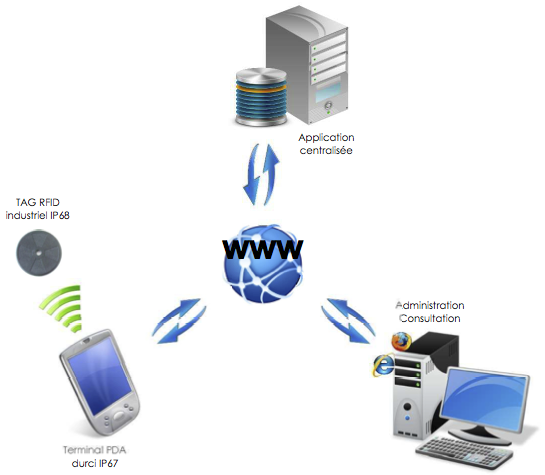
\includegraphics[scale=1.5]{images/gema.png}
    \caption{Ceci représente l'utilisation de GeMa via le réseau
    Internet. Dans le cadre du déploiement chez Syngenta, le serveur Web
    est remplacé par IITAMP en local chez le client.}
    \label{gema}
  \end{center}
\end{figure}
% section Présentation de GeMa (end)%}}}

\section{Mise en place de la solution} % (fold)%{{{
\label{sec:Mise en place de la solution}

Pour une interconnexion entre les sites, un dispositif de sécurité
impressionnant à été mis en place par Syngenta. En effet, ceux-ci
utilise la technologie VPN,\footnote{\emph{Virtual Private Network} ou
réseau privé virtuel.} qui permet d'obtenir une liaison sécurisée à
moindre coût.

Le réseau privé virtuel vise à apporter certains éléments essentiels
dans la transmission de données : l'authentification (et donc
l'identification) des interlocuteurs et la confidentialité des données via
le chiffrement (qui vise à les rendre inutilisables par quelqu'un
d'autre que le destinataire). La figure~\ref{vpn} illustre le principe
de ce type de connexion.

La mise en \oe{}uvre d'IITAMP ainsi que de GeMa s'effectuant dans
l'usine de Nerac près de bordeaux, le client nous à prêter un ordinateur
portable avec tout les outils nécessaire à la connexion à distance pour
éviter de me déplacer de Dunkerque jusqu'au site, ce qui représente à
peu près six cent kilomètres...

\begin{figure}
  \begin{center}
    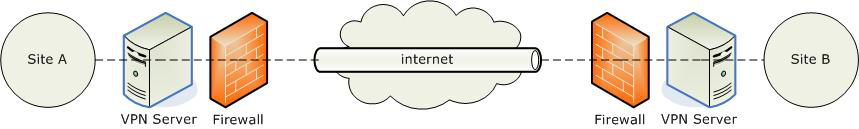
\includegraphics[scale=0.5]{images/vpn.png}
    \caption{Exemple de réseau privé virtuel entre deux sites.}
    \label{vpn}
  \end{center}
\end{figure}

\subsection{Harmonisation des systèmes d'informations} % (fold)%{{{
\label{sub:Harmonisation des systèmes d'informations}

Dans le cadre de cette mise en \oe{}uvre, le client veut récupérer les
données des interventions qui sont stockés dans la base MySQL de GeMa
dans leur système d'information qui possède une base de donnée SQL
Server. Cette duplication de donnée permet une intégration des
informations récoltés par GeMa dans le SI de l'entreprise à des fins de
traçabilité, ce qui permet à partir des autres logiciels du client de
faire des statistiques de production.

Pour cette duplication, il a fallu que je développe un script PHP qui
tout d'abord interroge la base de donnée de GeMa pour récupérer les
données, qui ensuite traite ses données pour les rendre compatibles à la
structure de la base du client ainsi qu'a la technologie SQL Server
utilisée et qui enfin insère ses données traités dans la base du client.

\subsection{Les tests} % (fold)%{{{
\label{sub:Les tests}

Comme nous l'avons vu, GeMa utilise la mobilité pour le rapport des
interventions. Pour tester si l'application GeMa fonctionne correctement
ainsi que le script de duplication de donnée, quelques tests furent
nécessaire. Sachant que le site de production n'est pas proche,
l'utilisation d'un émulateur de PDA au travers du réseau VPN fut
nécessaire.

Quelques problèmes sont apparu pendant la phase de debogage :
\begin{description}

  \item[Communication entre les bases :] XAMPP par défaut ne permet pas
    d'utiliser une base SQL Server, il à fallut que j'installe et
    configure le driver officiel de l'entreprise
    Microsoft pour permettre l'accès à la base de
    données.

  \item[Synthaxe invalide pour SQL Server :] Une habitude est ancrée
    dans l'utilisation du logiciel libre MySQL qui est de forcer
    l'encodage des caractères en UTF-8 afin d'éviter de futur problèmes.
    Cette manipulation ce fait via une requête SQL que l'on place dans
    le constructeur de la classe qui sert à instancier l'objet de
    connexion à la base de données. Comme les habitudes ont la vie dure,
    j'ai copié/collé un constructeur sans y prêter attention, cependant
    SQL Server ne connait pas cette syntaxe SQL. GeMa étant pourvu d'un
    système d'alerte par mail, M.~Dubourg recevait un courriel à 5
    minutes d'intervalles lorsque l'émulateur d'assistant personnel
    lançait la synchronisation distante avec le serveur\,
    \footnote{fonction de synchronisation automatique de GeMa Mobile
    lorsque il est sur son socle.}, sont client mail à bien entendu
    déplacer l'expéditeur entant que spam au bout de plusieurs reprises.
    Ne fermant pas l'émulateur la nuit pour éviter d'avoir à le
    relancer, une quantité impressionnante de mail m'a été annoncé
    quelques jours plus tard lorsque le cogérant à inspecté sa boite à
    pourriels.

  \item[Obligation de renseigner tous les champs :] L'ancien système de
    relevés ce faisant à l'aide d'un papier/crayon puis par l'ajout de
    ses annotations dans un fichier Excel, lorsqu'un champ n'avait
    aucune valeur, un zéro lui était attribué. En inspectant les données
    de la base SQL Server, je me suis rendu compte que mon script quant
    à lui n'insérait rien lorsqu'il n'y avait pas de valeur. J'en ai
    déduit qu'aucune règle de gestion n'avait été crée afin d'empêcher
    la non-saisi. J'ai donc été obligé d'inscrire cette règle via le
    code\,\footnote{c'est la base du client, je n'ai pas à intervenir
    dessus même si elle me parait mal conçu.} alors que la bonne méthode
    est habituellement de le faire via une option lors de la création de
    la base.

\end{description}
% subsection Les tests (end)%}}}
% subsection Harmonisation des systèmes d'informations (end)%}}}
% chapter Mise en oeuvre d'IITAMP (end)


\chapter{Conclusion} % (fold)
\label{cha:Conclusion}

\lettrine{L}{a} première chose qui me vient à l'esprit est la
progression que m'ont apporté ces stages. Je peux dire en toute
humilité que j'en ressors grandi.

J'ai pu m'appercevoir que l'entreprise utilisait toujours les
technologies que j'ai mis en place durant la première année, des
modifications ont été apportées mais mon code de base est toujours là,
ce qui indique une certaine qualité dans le travail que j'ai pu
accomplir.

J'ai continué de former les développeurs sur Git pour qu'ils aillent
toujours plus loin dans l'exploitation de celui-ci. En effet, j'avais
constaté dès la première semaine du deuxième stage que quelques
principes fondamentaux d'utilisation avaientt été oubliés. J'ai pu aussi
leur présenter de nouvelles fonctionnalités qui sont apparues pendant le
laps de temps entre les deux stages. L'usage de base convient dans
90\%{} des cas mais certaines particularités sont toujours bonnes à
connaître.

J'ai découvert le travail de développeur en entreprise et je dois dire
que cela me plaît, cependant ce n'est pas toujours évident.  Bloquer sur
un problème toute la journée sans avancer est très pénible
intellectuellement, j'ai connu beaucoup de maux de tête et de matins
difficiles. Travailler toute la journée à concevoir des algorithmes est
parfois éprouvant\dots

J'ai été très satisfait des échanges que j'ai pu avoir avec l'équipe.
Développer est une chose mais proposer, débattre, trouver les meilleures
solutions sont ce que j'ai préféré. L'entreprise m'a beaucoup apporté,
mais je pense aussi avoir apporté des choses et c'est très gratifiant.

Cette période m'a prouvé que je ne m'étais pas trompé dans mon
orientation. Je souhaite continuer mes études vers une licence
professionnelle systèmes informatiques et logiciels option \og
Développement et Administration de sites Internet et Intranet \fg{} qui
permettra de me spécialiser dans le Web et la sécurité, qui sont des
marchés porteurs autant dans les entreprises publiques que privées,
avant de m'insérer dans le monde du travail.
% chapter Conclusion (end)


% fake annexe
\appendix

\chapter{Attestation de stages} % (fold)
\label{cha:Attestations de stages}
1\iere{} \newpage
2\ieme{} \newpage
% chapter Attestations de stages (end)

\chapter{Intitulé des actions} % (fold)
\label{cha:Intitulé des actions}
% chapter Intitulé des actions (end)

\end{document}%}}}
